\subsection{Data}\label{subsec:data}
In the empirical analysis, we consider the risk reduction capability
of CME Bitcoin Futures (BTCF) on five cryptos, namely Bitcoin (BTC), Ethereum
(ETH), Cardano (ADA), Litecoin (LTC) and Ripple (XRP), as well as five
crypto indexes, namely BITX, BITW100, CRIX, BITW20, and BITW70.
ETH, ADA, LTC, and XRP are popular cryptos tradable in various
exchanges and have large market capitalization. 
BITX, BITW100, and CRIX are market-cap weighted crypto indexes with
BTC as constituent. 
BITX and BITW100 track the total return of the 10 and 100 cryptos
with largest market-cap, respectively. 
CRIX decides the number of constituents by AIC and tracks that number
of cryptos with largest market-cap. In our case, the number of
constituents in CRIX is 5. 
BITW20 is also a market-cap weighted crypto index but with the 20
largest market-cap cryptos outside the constituents of BITX.
BITW70 has the same construction as BITW20 but with the 70 largest
market-cap cryptos outside BITX and BITW20. 
Therefore, BTC is excluded as a constituent in BITW20 and BITW70.

For each of the 10 hedging portfolios, a crypto or index is considered
as the spot and held in a unit size long position, while 
the front BTCF is held in a short position with units corresponding to
the OHR in order to reduce the risk of the spot. 
Except for the hedge of BTC, all hedging portfolios are considered to
be cross-asset hedges. 

We collect the spots' and BTCF's daily prices at 15:00 US Central Time
(CT). The reason for choosing this particular time is that the CME
group determines the daily settlements for BTCF's based on the trading
activities on CME Globex between 14:59 and 15:00 CT. This is also the
reporting time of the daily closing price by Bloomberg. 
The crypto spot data is collected from the data provider called
Tiingo (\href{https://www.tiingo.com/}{https://www.tiingo.com/}).
Tiingo aggregates crypto OHLC (open, high, low, and close) prices fed
by APIs from various exchanges. It covers major exchanges, such as
Binance, Gemini, Poloniex etc., so Tiingo's aggregated OHLC price is a
good representation a tradable market price. 
For each crypto, we match the opening price at 15:00 CT from Tiingo
with the daily BTCF closing price from Bloomberg.
Since CRIX is not available at 15:00 CT, we recalculated an hourly
CRIX using the monthly constituents weights and the hourly OHLC price
data collected from Tiingo. 
BITX, BITW20, BITW70, and BITW100 are collected from the official
website of their publisher Bitwise.com. 
The daily reporting time of the Bitwise indexes is 15:00 CT.

At the time of writing, the CRIX is undergoing the listing process on
the S\&P Dow Jones Indices, the official CRIX data will then be
calculated with Lukka Prime Data and available to the public via S\&P.

\subsection{Overview of the out-of-sample data}\label{subsec:oosdata}

For every asset and hedge portfolio, we concatenate the out-of-sample data to form a time series for analysis.
The date range of the out-of-sample time series is from 2019-10-21 to 2021-05-27, in total of 405 data points in each time series.
We analyse these time series throughout the whole result section. 

We introduce the out-of-sample data in this subsection before we proceed to analysing the hedged portfolio results.
Figure~\ref{fig:BTC_price} presents the BTC and BTCF price in USD in the first panel and the arithmetic difference between the daily return of BTC and BTCF, i.e. $R_s - R_f$, in the
second panel.
In the first panel, the black vertical lines with capital letter labels indicate the days of the five most negative daily return of BTC during out-pf-sample period.
Table \ref{tab:BTC_5min} summarizes the relevant news headlines and events of those days. 

Figures~\ref{fig:index_price} and \ref{fig:individualCoins_price} are the cumulative returns of the indices and individual cryptos respectively.
The black vertical lines labeled by assets name are the largest daily price drop of the assets in the out-of-sample data. 

The out-of-sample data covers the pre-COVID19 period, 2019-10-21 to 2020-03-09, as well as the COVID19 period, 2019-03-19 onwards.
We can observe an overall upward trend of crypto prices in both periods.
Nonetheless, the volatilities of assets are high (annualized around 100\%) regardless of COVID19.

%\newpage
\begin{figure}[t]
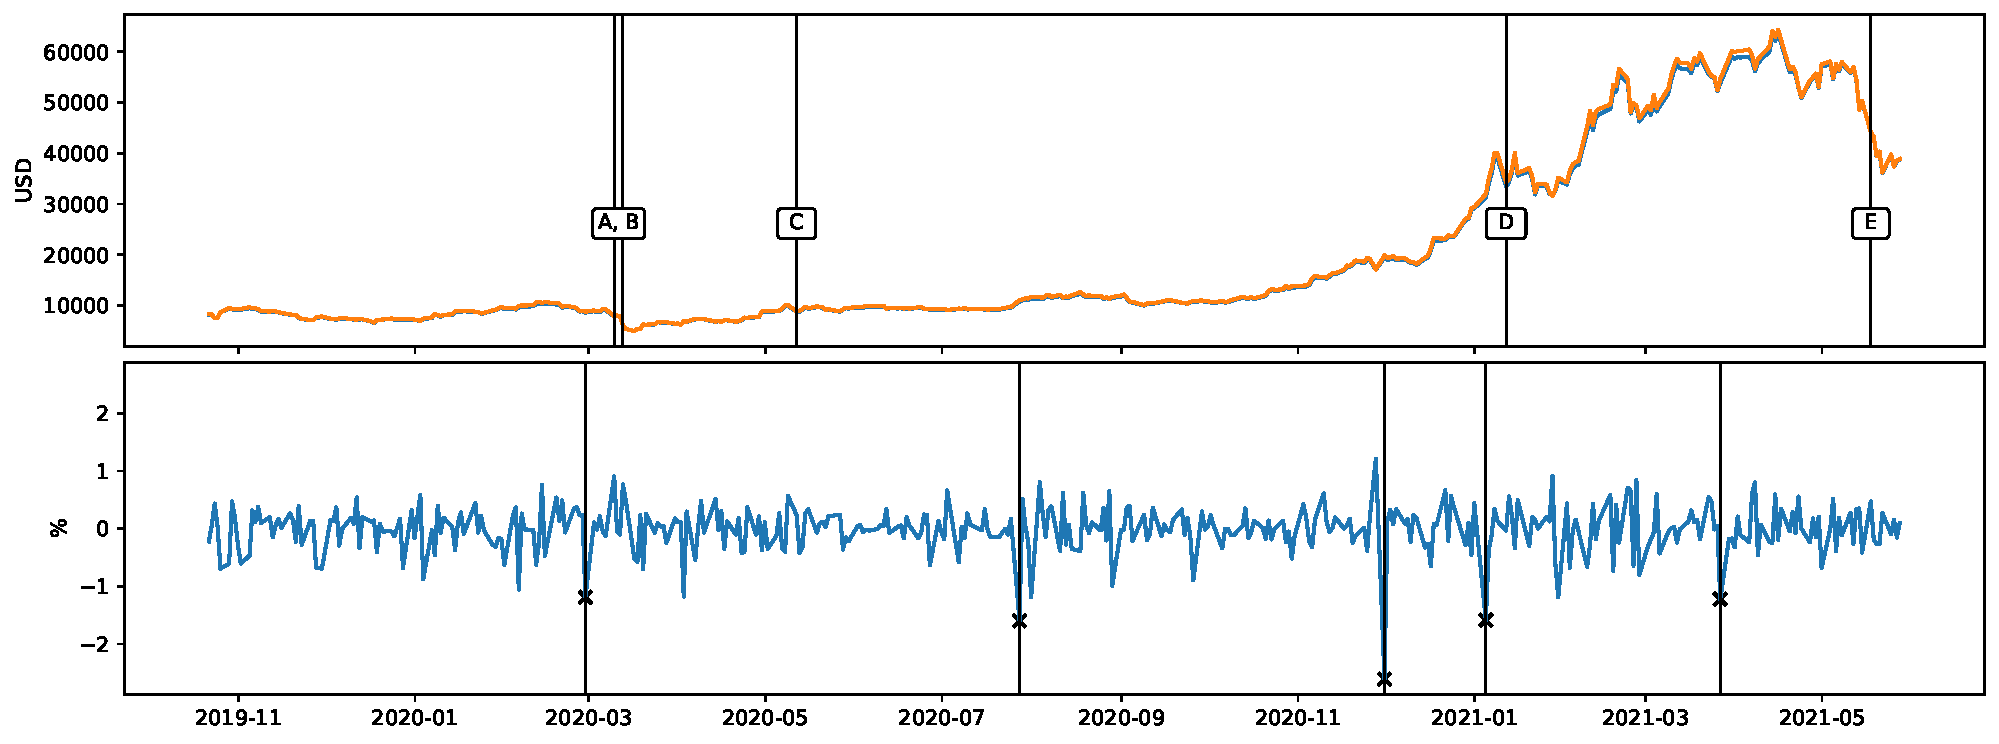
\includegraphics[width=\textwidth]{_pics/BTC_price.pdf}
  \caption{Out-of-sample BTC and BTCF price. The first panel presents the price of BTC in blue line and that of BTCF in orange line.
  The black vertical lines with capital letter labels indicate the five most negative daily return of BTC in the out-of-sample data.
  The second panel presents the difference between the \% return of BTC and BTCF.
  The black vertical lines indicate the five most negative returns.
  The crosses locate the level the returns.}
%  \href{http://www.quantlet.com/}{\includegraphics[height=\baselineskip]{_pics/qletlogo_tr.png}} }
\label{fig:BTC_price}
\end{figure}

\begin{table}[!h]
    \centering
      \begin{tabularx}{.8\textwidth}{cccX}
        \toprule
        Label &   Date & \% Drop in Price &  Summary\\
        \midrule
        A &  2020-03-09 & 13.83 &  Coronavirus outbreak that affect the global markets; BTC as potential safe-haven was questioned.$^1$\\
        B &  2020-03-12 & 22.89 &  Continuation of the 2020-03-09 drop.  \\
        C &  2020-05-11 & 12.11 &  Price correction (from \$10,000 to \$8,100) after BTC price surge because of the third supply halving.$^{2,3}$ \\
        D &  2021-01-11 & 14.41 &  Short term correction of BTC hits the \$40,000 mark.$^4$\\
        E &  2021-05-17 & 11.86 &  Tesla stopped taking BTC as payment due to environmental concerns about energy use to process transaction.$^5$\\
        \bottomrule
      \end{tabularx}
        \caption{Summary of events that associated with the five most negative daily price drops in out-of-sample BTC price data.
        The capital letter labels in the first column are the labels in the first panel of figure~\ref{fig:BTC_price}.
        $^1$ is reported by the CNBC news \url{https://cnb.cx/3HZ2x7K}; $^2$ is from Forbes \url{https://bit.ly/3rdJPmP};
        $^3$ is from livemint.com \url{https://bit.ly/3FRi6Na};
        $^4$ is from CNBC \url{https://cnb.cx/3nU0ppO};
        $^5$ is from Reuters \url{https://reut.rs/3leCiAv}.
        }
        \label{tab:BTC_5min}
  \end{table}

%\clearpage

%\newpage
\begin{figure}[t]
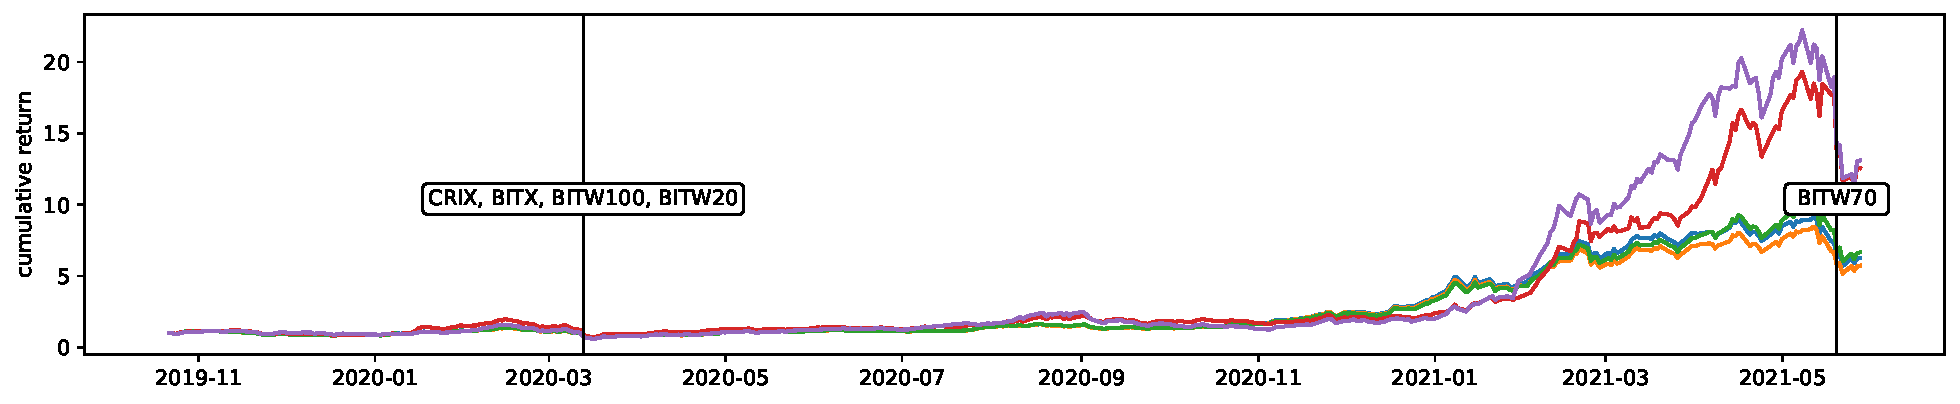
\includegraphics[width=\textwidth]{_pics/index_price.pdf}
  \caption{Out-of-sample cumulative return of crypto indices.
  The black vertical lines indicate largest price drop of indices indicated by the labels.
  The colouring is as follows:
  \textcolor{plt1}{Blue line} is CRIX;
  \textcolor{plt2}{Orange line} is BITX;
  \textcolor{plt3}{Green line} is BITW100;
  \textcolor{plt4}{Red line} is BITW20;
  \textcolor{plt5}{Purple line} is BITW70.
  }
%  \href{http://www.quantlet.com/}{\includegraphics[height=\baselineskip]{_pics/qletlogo_tr.png}} }
\label{fig:index_price}
\end{figure}

\begin{figure}[t]
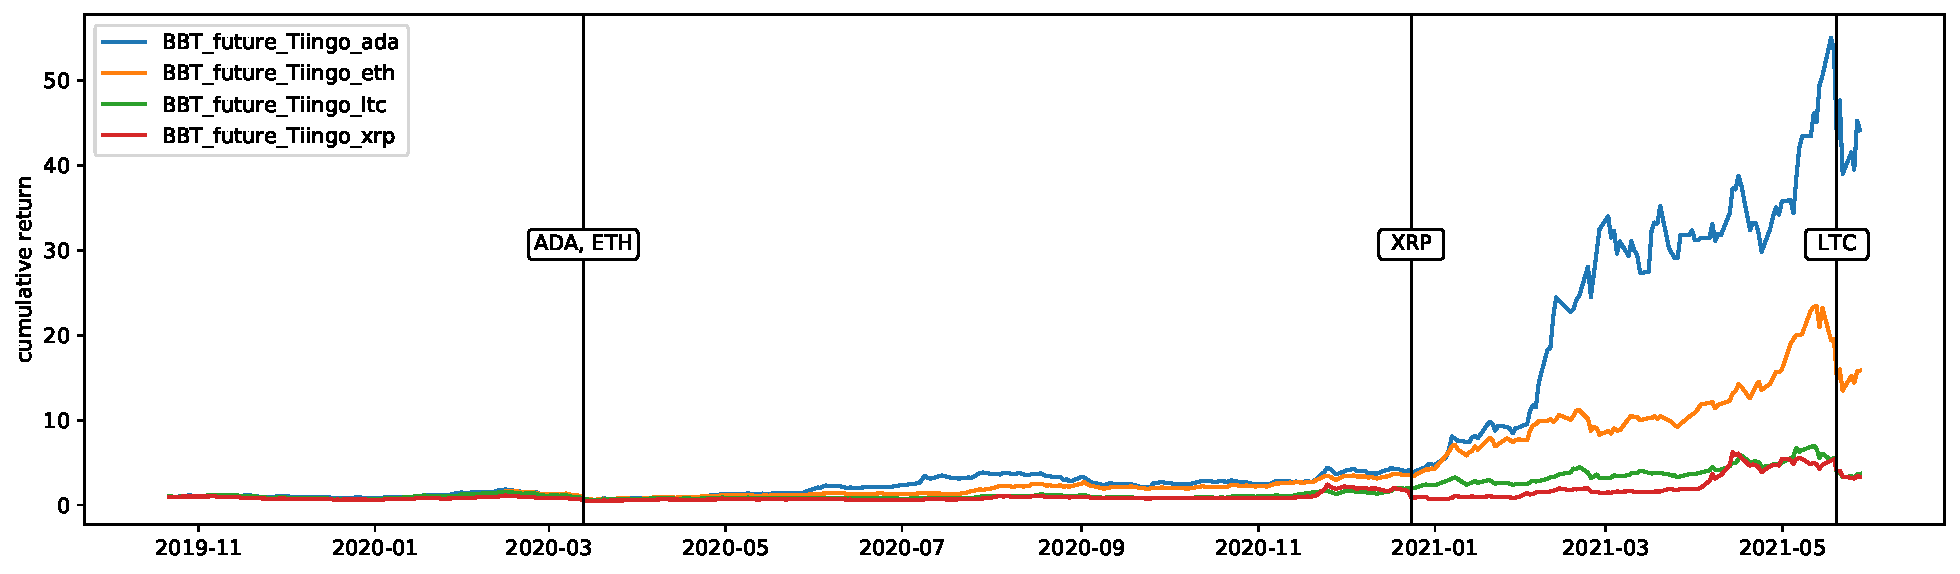
\includegraphics[width=\textwidth]{_pics/individualCoins_price.pdf}
  \caption{Out-of-sample cumulative return of individual cyptos.
  The black vertical lines indicate largest price drop of cryptos indicated by the labels.
    \textcolor{plt1}{Blue line} is ADA;
  \textcolor{plt2}{Orange line} is ETH;
  \textcolor{plt3}{Green line} is LTC;
  \textcolor{plt4}{Red line} is XRP.}

%  \href{http://www.quantlet.com/}{\includegraphics[height=\baselineskip]{_pics/qletlogo_tr.png}} }
\label{fig:individualCoins_price}
\end{figure}

\begin{table}[t]
    \centering
      \begin{tabularx}{.8\textwidth}{cccX}
        \toprule
        Label &  Date & \% Drop in Price &  Summary\\
        \midrule
        CRIX    &2020-03-09 & 23.77 & \multirow[t]{6}{\hsize}{Coronavirus outbreak that affect the global markets including the crpyto market.}\\
        BITX    & & 23.68 &  \\
        BITW100 & & 23.87 &  \\
        BITW20  & & 26.66 &  \\
        ADA     & &23.55 &  \\
        ETH     & &27.40 &  \\
        BITW70  & 2021-05-19& 27.64 & The spillover of the BTC shock on 2021-05-17 (label A in figure~\ref{fig:BTC_price} and table~\ref{tab:BTC_5min})\\
        XRP     & 2020-12-23 & 41.00 & Top executives were sued by the SEC of misleading investors$^1$. \\
        \bottomrule
      \end{tabularx}
        \caption{Summary of events that associated with largest price drops in out-of-sample data.
        The labels in the first column are the labels in figure \ref{fig:index_price} and figure \ref{fig:individualCoins_price}.
        CRIX, BITX, BITW100, BITW20, ADA and ETH have the same date the reason of the largest drop. $^1$ is reported by Bloomberg \url{https://bloom.bg/3cWdita}.}
        \label{tab:All_min}
  \end{table}
%\clearpage


%%% Local Variables:
%%% mode: latex
%%% TeX-master: "SRM"
%%% End:
